% !TeX spellcheck = en_GB
\chapter*{Introduction}
	\addcontentsline{toc}{chapter}{Introduction}
	\markboth{Introduction}{}
	\textcolor{red}{Das ist wohl etwas zu dick aufgetragen.}

	In this thesis, we introduce a damped wave equation to model the mechanistic behavior of a cardiomyocyte on the level of its sarcomeres. 


	As in any field of abstraction, an observer makes a, more or less, accurate observation of reality. This observation might be considered as a phenomena, that one is interested in researching further. The thinking mind comes into play by producing some kind of \textit{idea}, that is, a mechanism that encapsulates the occurence of the phenomena one is interested in. Thorougly speaking, we call this idea \textit{a model}. A model has the notable property to generate \textit{predictions}.

It is notable to mention, that any observation and any model of reality  has some quirks. However, there are some models, whose fit to the observed data is satisfactory; and even more compelling the leaner the model is. A model many people might recognize is,

\begin{equation*}
	F_g = G \frac{m_1 \ m_2}{r^2},
\end{equation*}

the Law of Gravity. Here, the parameter that had to be fitted was the gravitational constant
\begin{equation*}
	G  \sim 6,67 \ 10^{-11} \frac{m^3}{kg \ s^2}
\end{equation*}
The model impresses by consisting of only three variables. However, the predictions it generates for everyday purposes are overshadowed only by the lacking quality of its observations.

In this case, it is said that the observer sat below a tree watching an apple fall down, when suddenly the idea of the model arose.





In the paper  introduce a sublinear operator on the class of bounded continuous functions that can be thought of as a generalized expectation. They prove that this operator is a viscosity solution to an associated partial differential equation. To prove this, they rely on an optimality property that the operator satisfies. We call this property \emph{dynamic programming principle} (DPP). The DPP formalizes the idea that for a value function to be optimal in a dynamic system, it is necessary and sufficient, if we
\begin{itemize}
	\item consider it starting from a future point in time $t > 0$ in an arbitrary state and find an optimal control starting there;
	\item optimize over the whole time horizon for the reduced problem, which, starting at time $t$, uses the above optimal controls.
\end{itemize}
For papers in a similar framework, the dynamic programming principle is often the backbone of such work 

This thesis happens in a similar setting. We take the same approach as  for a slightly different operator which will be convex and not sublinear. Our main focus will be to retrace their proof of the viscosity solution in our case. A key property that we aim to establish in this way is domain invariance. Thus we work towards showing that continuous bounded functions are mapped to such. Establishing this so called $\mathcal{C}_b$-\emph{Feller}-property enables us to look at the convex expectation as a semigroup on the time interval.

Aside from studying these regularity properties, we address the question of wether our solution is unique. We investigate if under certain conditions, uniqueness at the level of viscosity solutions carries over to the level of semigroups. \newpage


	\subsection*{Acknowledgements}
I acknowledge the use of OpenAI’s ChatGPT (version 5.2) for assistance with phrasing suggestions, improving the readability of the text, and generating LaTeX code for the figures included in this thesis.

All analyses, interpretations, and conclusions presented in this report are entirely my own.

% Lastly, it remains a pleasant duty to thank Prof. Dondl for insightful talks within the field of elasticity theory.

\subsection*{Notation}


\begin{comment}
		\vspace*{-.5cm}
		Let $F=(F^1, \dots, F^d): D \rightarrow Im \subset \mathbb{R}^d$ be a continuously differentiable vector field. We will use the following notation: \par
		\begin{table}[H]
			\flushleft
			\begin{tabularx}{\textwidth}{@{}cX@{}}
				$ \nabla F = (\partial_1 F, \dots, \partial_d F)$ & The Gradient of $F$. \\
				$ \operatorname{Div} F = \nabla \cdot F = \sum_{i=1}^{d} \partial_i F^i $ & The Divergence of $F$. \\
				$ \Omega$ & Continuous functions from $ \mathbb{R}_{\geq 0}$ to $\mathbb{R}^d $. \\
				$ \omega( \cdot ) $ & An element of $\Omega $. \\
				$ \rho= \rho(x, t) > 0 $ & Die Massendichte eines Punktes $x$ zur Zeit $t$. Es gilt $dm = \rho dV$ für Volumen und Masse.\\
				$ \mathbf{F} = \left[ \nabla_{\mathbf{a}} \mathbf{x}(\mathbf{a}, t) \right]^{T}$ & Der Deformationsgradient im Punkt $a$.
				$ X = X(x,t) $ & Lagrangsche Koordinaten. Materialpunktabbildung. Welcher Punkt $X$ ist zur Zeit $t$ and Ort $x$?
				$ x = x(X,t) $ & Eulersche Koordinaten. Bewegungsabbildung. Wo ist Punkt $X$ zur Zeit $t$?
				$ (\mathcal{M}_{loc})$, $\mathcal{M} $ & (Local) martingales on $ \Omega $. \\
				$ \mathcal{V}$ & Finite variation processes on $ \Omega $.\\
				$ \mathcal{V}_+$ & Increasing processes on $ \Omega $.\\
				$ \mathcal{C}^{\infty}_b(\mathbb{R}^d)$ & The class of bounded continuous functions from $\mathbb{R}_+$ to $\mathbb{R}^d$, infinetly differentiable where all derivatives are bounded. \\
				$\| \cdot \| $ & The supreme norm, if not specified else. \\
				$ A^* $ & The transpose of a matrix $ A $. \\
				$\operatorname{tr}[ A ] $ & The trace of a matrix $ A $. \\
				$\| A \|_{F} $ & The Frobenius norm of a matrix $ A $. $\| A \|_{F} := \sqrt{\operatorname{tr}[A^* A]}$. \\
				$ \mathcal{F} $ & The natural filtration of the canonical process. \\
				$ \mathcal{P} $ & The progressive $\sigma$-field. \\
				$ H \cdot M $ & The stochastic Integral of $H$ with respect to $ M $. \\
				$ dH_s $, $H_s \ d M_s$ & $H_s - H_0$ and the stochastic intragral of $ (H \cdot M)_s $.\\
				$ \langle M, N \rangle $ & The quadratic covariation process of $ M $ and $ N $. \\
				$ W $ & A $d$-dimensional Brownian Motion. \\
				$ A \twoheadrightarrow B$ & A correspondence, i.e. a mapping from a set $ A $ to the powerset of $ B $.
			\end{tabularx}
		\end{table}
\end{comment}




\section{2 D Federmodell}
\textcolor{red}{bitte über die Modellannahmen eifrig diskutieren}. Das Setting hier ist in Anlehnung an das Kapitel "Punkte und Vektoren" auf Seite 203 von \cite{EckGarcke2017}. Sei $E^3$ der euklidische Raum, $\mathcal{V}$ der \textit{zugehörige?} $\mathbb{R}$- Vektorraum mit euklidischem Skalarprodukt $u \cdot v, \quad u,v \in \mathcal{V}$ und sei $(e_1, e_2, e_3)$ eine Orthonormalbasis von $\mathcal{V}$. \newline 
Nach Auswahl eines Ursprungs $\mathcal{O} \in E^3$ lässt sich die Orthonormalbasis $(e_1, e_2, e_3)$ zu einem Koordinatensystem in $E^3$ ergänzen. Ein Punkt $x=(x_1, x_2, x_3) \in E^3$ hat dann die Koordinaten:
\begin{equation*}
	x_i = (x-\mathcal{O}) \cdot e_i
\end{equation*}
\textcolor{red}{ist das wohldefiniert? Von wo nach wo geht diese Abbildung?}. Ja. $x_i - \mathcal{O}$ ist als Differenz von zwei Punkten aus $E^3$ ein Vektor und damit ist das ein wohldefiniertes Skalarprodukt. Der Punkt $x$ ist dann als Abstand vom Ursprung um den Koordinatenvektor aufzufassen. Diese Koordinaten beschreiben also den Ort von $x$ innerhalb des Vektorraumes mit $\mathcal{O}$ als Ursprung. \newline 

Damit wir nicht Gefahr laufen irrtümlicherweise Operationen wie $x+y, \quad x,y \in E^3$ aufzuschreiben, möchte ich daran erinnern, dass wir $E^3$ hier nicht als Vektorraum verstehen, sondern als eine Menge von Punkten die über $\mathcal{O}$ kanonisch isomorph zum R3 sind. Erlaubt sind demnach formalismen wie
			\begin{tabularx}{\textwidth}{@{}cX@{}}
				$ x-y=u \in \mathcal{V}$ & den Verschiebungsvektor von $x-y$. \\
				$ x+u=y \in E^3$ & das Verschieben von $x$ um den Vektor $u$. \\
			\end{tabularx}
	




\subsection*{Mechanistic cell model}

Wir betrachten Massepunkte $a_{ij} \in E^3$ die Z-Scheiben darstellen. Wir wählen als Ursprung die obere linke Z-Scheibe $\mathcal{O}:= a_{11}$. Weiterhin sei $u_{ij}(t) := a_{ij}(t) - a_{ij}(0)$ die Verschiebung des Massepunktes $a_{ij}$.

Ihre Positionen \textcolor{red}{(hier im R3} sammeln wir in der Matrix $A$, die Verschiebungen in der Matrix $U$,
\begin{equation*}
	E^{3^{n \times m}} \ni A=
\begin{pmatrix}
a_{11} & a_{12} & \cdots & a_{1m} \\
a_{21} & a_{22} & \cdots & a_{2m} \\
\vdots & \vdots & \ddots & \vdots \\
a_{n1} & a_{n2} & \cdots & a_{nm}
\end{pmatrix}, U=
\begin{pmatrix}
u_{11} & u_{12} & \cdots & u_{1m} \\
u_{21} & u_{22} & \cdots & u_{2m} \\
\vdots & \vdots & \ddots & \vdots \\
u_{n1} & u_{n2} & \cdots & u_{nm}
\end{pmatrix}
\end{equation*}



Wir nehmen als Modellannahme für die Kräfte die auf die Massepunkte $a_{ij}$ wirken eine gedämpfte Schwingung.
\begin{equation*}
	F = F_F + F_R + f = m \ddot{u}
\end{equation*}
mit $u$ einem (Verschiebungs)vektor für einen Punkt bzw. allgemeiner als Vektorfeld. Jeder Punkt $a_{ij}$ erfährt zum Zeitpunkt $t$ also einen Kraftvektor $F_{ij}(t) \in \mathbb{R}^2$ der an $a_{ij}(t)$ ansetzt.


Hier ist $F_F$ gegeben durch das Hook'sche Gesezt, $F_R$ eine Reibungskraft und $f=f(t, ?)$ einer von außen wirkenden Kraft.

Based on the architecture of a striated muscle cell, we assume the following spring grid (Federgitter).

\begin{figure}[H]
    \centering

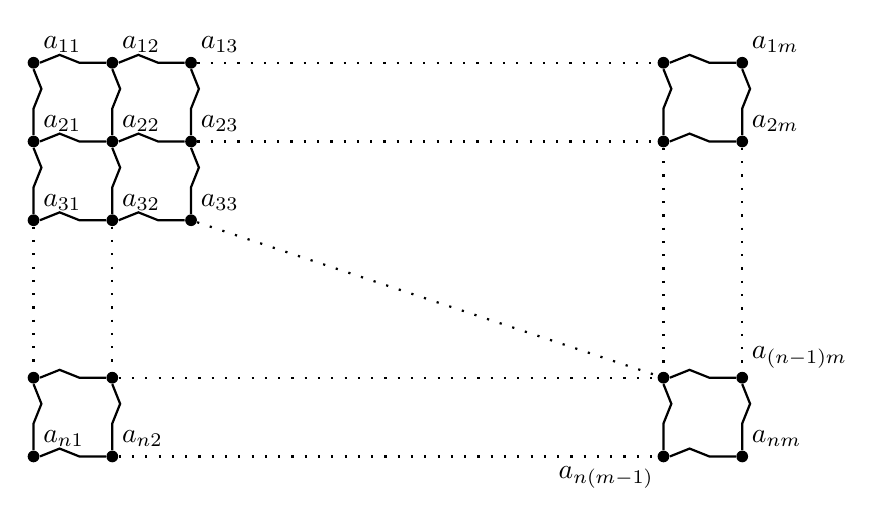
\begin{tikzpicture}[
    spring/.style={
        thick,
        decorate,
        decoration={zigzag,segment length=10mm,amplitude=1mm}
    }
]


%%%%%%%%%%%%%%%%%%%%%			 Massepunkte			Set: l=n-1		k=m-1		%%%%%%%%%%%%%%%%%
%erste Zeile
\node[circle,fill=black,inner sep=1.5pt]
    (a11) at (1,-1) {};
\node[above right] at (a11) {$a_{11}$};

\node[circle,fill=black,inner sep=1.5pt]
    (a12) at (2,-1) {};
\node[above right] at (a12) {$a_{12}$};

\node[circle,fill=black,inner sep=1.5pt]
    (a13) at (3,-1) {};
\node[above right] at (a13) {$a_{13}$};


\node[circle,fill=black,inner sep=1.5pt]
    (a1k) at (9,-1) {};

\node[circle,fill=black,inner sep=1.5pt]
    (a1m) at (10,-1) {};
\node[above right] at (a1m) {$a_{1m}$};

%Zweite Zeile
\node[circle,fill=black,inner sep=1.5pt]
    (a21) at (1,-2) {};
\node[above right] at (a21) {$a_{21}$};

\node[circle,fill=black,inner sep=1.5pt]
    (a22) at (2,-2) {};
\node[above right] at (a22) {$a_{22}$};

\node[circle,fill=black,inner sep=1.5pt]
    (a23) at (3,-2) {};
\node[above right] at (a23) {$a_{23}$};

\node[circle,fill=black,inner sep=1.5pt]
    (a2k) at (9,-2) {};

\node[circle,fill=black,inner sep=1.5pt]
    (a2m) at (10,-2) {};
\node[above right] at (a2m) {$a_{2m}$};

%Dritte Zeile
\node[circle,fill=black,inner sep=1.5pt]
    (a31) at (1,-3) {};
\node[above right] at (a31) {$a_{31}$};

\node[circle,fill=black,inner sep=1.5pt]
    (a32) at (2,-3) {};
\node[above right] at (a32) {$a_{32}$};

\node[circle,fill=black,inner sep=1.5pt]
    (a33) at (3,-3) {};
\node[above right] at (a33) {$a_{33}$};


%(n-1)-te Zeile
\node[circle,fill=black,inner sep=1.5pt]
    (al1) at (1,-5) {};

\node[circle,fill=black,inner sep=1.5pt]
    (al2) at (2,-5) {};

\node[circle,fill=black,inner sep=1.5pt]
    (alk) at (9,-5) {};

\node[circle,fill=black,inner sep=1.5pt]
    (alm) at (10,-5) {};
\node[above right] at (alm) {$a_{(n-1)m}$};

%n-te Zeile
\node[circle,fill=black,inner sep=1.5pt]
    (an1) at (1,-6) {};
\node[above right] at (an1) {$a_{n1}$};

\node[circle,fill=black,inner sep=1.5pt]
    (an2) at (2,-6) {};
\node[above right] at (an2) {$a_{n2}$};

\node[circle,fill=black,inner sep=1.5pt]
    (ank) at (9,-6) {};
\node[below left] at (ank) {$a_{n(m-1)}$};

\node[circle,fill=black,inner sep=1.5pt]
    (anm) at (10,-6) {};
\node[above right] at (anm) {$a_{nm}$};




%%%%%%%%%%%%%%%%%%%				SPRINGS				%%%%%%%%%%%%%%%%%%
\draw[spring] (a11) -- (a12);
\draw[spring] (a21) -- (a22);
\draw[spring] (a11) -- (a21);
\draw[spring] (a12) -- (a22);

\draw[spring] (a12) -- (a13);
\draw[spring] (a22) -- (a23);
\draw[spring] (a32) -- (a33);

\draw[spring] (a21) -- (a31);
\draw[spring] (a22) -- (a32);
\draw[spring] (a23) -- (a33);

\draw[spring] (a31) -- (a32);
\draw[spring] (a13) -- (a23);

%%%%%%%%%%%%%%%					Unten links					%%%%%%%%%%%%%
\draw[spring] (al1) -- (al2);
\draw[spring] (an1) -- (an2);
\draw[spring] (al1) -- (an1);
\draw[spring] (al2) -- (an2);


%%%%%%%%%%%%%%%%%%%					Oben Rechts				%%%%%%%%%%
\draw[spring] (a1k) -- (a1m);
\draw[spring] (a2k) -- (a2m);
\draw[spring] (a1k) -- (a2k);
\draw[spring] (a1m) -- (a2m);



%%%%%%%%%%%%%%%%%%%				Unten rechts			%%%%%%%%%%%%%%%%
\draw[spring] (alk) -- (alm);
\draw[spring] (alk) -- (ank);
\draw[spring] (alm) -- (anm);
\draw[spring] (ank) -- (anm);

\draw[loosely dotted, thick] (a13) -- (a1k);
\draw[loosely dotted, thick] (a23) -- (a2k);
\draw[loosely dotted, thick] (al2) -- (alk);
\draw[loosely dotted, thick] (an2) -- (ank);

\draw[loosely dotted, thick] (a33) -- (alk);

\draw[loosely dotted, thick] (a31) -- (al1);
\draw[loosely dotted, thick] (a32) -- (al2);
\draw[loosely dotted, thick] (a2k) -- (alk);
\draw[loosely dotted, thick] (a2m) -- (alm);

\end{tikzpicture}		
    \caption{Spring model of a cardiomyocyte}
\end{figure}

The nomenclature of the springs is as follows. Springs modeling \textit{sarcomeric}, that is inter Z-disk forces are subsumed under the index $l$. The spring coefficient $l_{i,j}$ belongs to the spring going from mass point $a_{i,j}$ to mass point $a_{i,j+1}$. Likewise, springs modeling vertical \textit{non-sarcomeric} inter Z-disk interaction are subsumed under the index $k$.  Hence, $k_{i,j}$ ist the spring coefficient of the spring going from mass point $a_{i,j}$ to mass point $a_{i+1,j}$. Note that, in the following the vertical springs are assumed \textbf{not actively contracting} whereas the sarcomeric springs are.

\begin{figure}[H]
    \centering

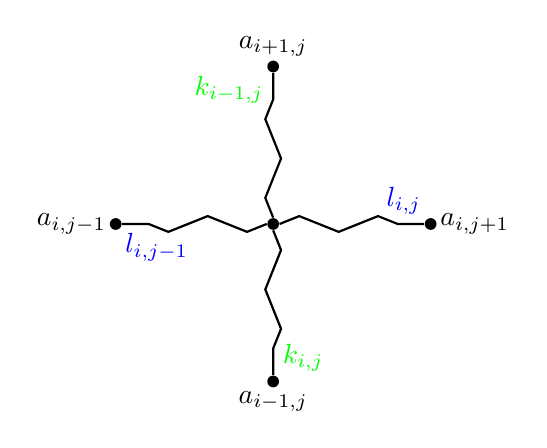
\begin{tikzpicture}[
    spring/.style={
        thick,
        decorate,
        decoration={zigzag,segment length=10mm,amplitude=1mm}
    }
]


%%%%%%%%%%%%%%%%%%%%%			 Massepunkte			Set: l=n-1		k=m-1		%%%%%%%%%%%%%%%%%
%erste Zeile
\node[circle,fill=black,inner sep=1.5pt]
    (aij) at (0,0) {};
%\node[above right] at (aij) {$a_{i,j}$};

\node[circle,fill=black,inner sep=1.5pt]
    (auj) at (2,0) {};
\node[right] at (auj) {$a_{i,j+1}$};
\node[above left, blue] at (auj) {$l_{i,j}$};

\node[circle,fill=black,inner sep=1.5pt]
    (aoj) at (-2,0) {};
\node[left] at (aoj) {$a_{i,j-1}$};
\node[below right, blue] at (aoj) {$l_{i,j-1}$};

\node[circle,fill=black,inner sep=1.5pt]
    (aik) at (0,2) {};
\node[above ] at (aik) {$a_{i+1,j}$};
\node[below left, green] at (aik) {$k_{i-1,j}$};

\node[circle,fill=black,inner sep=1.5pt]
    (aih) at (0,-2) {};
\node[below ] at (aih) {$a_{i-1,j}$};
\node[above right, green] at (aih) {$k_{i,j}$};


\draw[spring] (aij) -- (auj);
\draw[spring] (aij) -- (aoj);
\draw[spring] (aij) -- (aik);
\draw[spring] (aij) -- (aih);

\end{tikzpicture}		
\caption{Spring coefficients neighbouring Z-disk $a_{i,j}$.}
\end{figure}


We collect the spring coefficients in two matrices.
\begin{equation*}
	K=
\begin{pmatrix}
k_{11} & k_{12} & \cdots & k_{1m} \\
k_{21} & k_{22} & \cdots & k_{2m} \\
\vdots & \vdots & \ddots & \vdots \\
k_{(n-1)1} & k_{(n-1)2} & \cdots & k_{(n-1)m}
\end{pmatrix}, 
\qquad L = \begin{pmatrix}
l_{11} & l_{12} & \cdots & l_{1(m-1)} \\
l_{21} & l_{22} & \cdots & l_{2(m-1)} \\
\vdots & \vdots & \ddots & \vdots \\
l_{n1} & l_{n2} & \cdots & l_{n(m-1)}
\end{pmatrix}.
\end{equation*}

\newpage

Zurück zu den Kräften die an einer Z-Scheibe $a_{ij}$ ansetzen: Sei
\begin{equation*}
	u_{k_{ij}} := \text{ Neutralllänge der Feder } k_{ij}, \qquad u_{l_{ij}} := \text{ Neutralllänge der Feder } l_{ij} \quad \in \mathbb{R}
\end{equation*}

Damit gilt für die Federkraft der $l_{i,j}$-en (bzw. $k_{i,j}$-en) Feder
\begin{equation*}
	F_{F_{l_{ij}}} = l_{ij} \big(\|a_{i,j+1}(t) - a_{i,j}(t)\| - n_{l_{ij}} \big) \ \ \frac{a_{i,j+1}(t) - a_{i,j}(t)}{\|a_{i,j+1}(t) - a_{i,j}(t)\|} \hfill \in \mathbb{R}^2
\end{equation*}
Diese Federkraft wirkt zum Zeitpunkt $t$ zwischen den Punkten $a_{i,j}$ und $a_{i,j+1}$ mit Newtons dritten Axiom als Kraft und Gegenkraft.


Über die Summe der vier angrenzenden Federn erhalten wir den Federkraftvektor
\begin{equation*}
		F_{F_{i,j}}(t) = F_{F_{l_{i,j-1}}} - F_{F_{l_{i,j}}} + F_{F_{k_{i-1,j}}} - F_{F_{k_{i,j}}}
\end{equation*}

Nun für die Reibungskraft: $F_R = -\beta \dot{u}$, wobei man $\beta$ z.B. stocke'sch wählen kann. 
Für die Reibungskraft wäre es besser eine Deformationsmartrix zu nehmen um zu schauen wie sich die Dichte lokal verändert.

Letzlich modellieren wir eine äußere Kraft. Hier ist die Frage ob man diese explizit an die Zeit koppelt, oder ob man sie an Calcium koppelt und implizit über einen periodischen Calciumtransienten einbettet. Wir gehen hier mal den zweiten Weg: $f: \mathbb{R}_+ (Calcium) \rightarrow \mathbb{R}$. Wir wählen die Kontraktionskraft hier wieder als \textit{skalare} Größe die Entlang der $l_{i,j}$ Federn wirkt. Die Richtung erfährt sie also über die Lage der Feder zwischen $a_{i,j}$ und $a_{i,(j+)}$. Um Lesions zu modellieren erlauben wir in jedem Sarkomer eine eigene Funktion für die Kontraktionskraft.

Weiterhin möchten wir, dass ein Anstieg der Kontraktionskraft damit einhergeht, dass Calcium gebunden wird, das heißt, Calcium aus 
\begin{equation*}
	F_{contract_{l_{i,j}}}(Ca)
\end{equation*}

Um eine Rückkopplung mit dem Calcium zu erreichen, formalisieren wir folgenden Gedanken \textit{ist die Kontraktionskraft $f$ an einem Sarkomer hoch, und wirken überdies zugkräfte die das sarkomer auseinanderziehen, so wird vom gebundenen calcium wieder welches frei}





Wir erhalten aus dem Newtonschen Gesetz $F= m \ddot{u}$
\begin{equation*}
	F = F_F + F_R + f = m \ddot{u} \Leftrightarrow \ddot{u}(t) + 2a \dot{u} + bu(t) = g(t)
\end{equation*}
wobei $a = \frac{\beta}{2m}, b = \frac{k}{m}, g(t)=\frac{f(t)}{m}$.

\newpage

\section{Herleitung der Differentialgleichung zur linearen Elastizitätstheorie}

Die Differentialgleichung die wir zur Modellierung verwenden werden leitet sich her aus dem Impulserhaltungs und dem Energieerhaltungssatz. Daraufhin folgen zwei Linearisierungsschritte. Seien

\begin{enumerate}[label=\roman*)]
	\item $\varrho: \mathbb{R}_+ \times \Omega \rightarrow \mathbb{R} \ [\frac{m}{V}]$ die volumenbezogene Massedichte,
	\item $f: \Omega(t) \rightarrow \mathbb{R}^d \ [\frac{F}{m}]$ eine \textit{massenbezogene} Kraftdichte,
	\item $b: \partial \Omega(t) \rightarrow \mathbb{R}^d \ [\frac{F}{A}]$ eine \textit{Oberflächenbezogene} Kraftdichte,
	\item $e: \mathbb{R}_+ \times \Omega \rightarrow \mathbb{R}_+ \ [\frac{E}{V}]$ die volumenbezogene Dichte der \textit{elastischen Energie}.
\end{enumerate}


Newton's zweiter Hauptsatz besagt
\begin{equation*}
	\text{Kraft } = \text{Masse } \text{Beschleunigung}
\end{equation*}
bzw. mit unserer Notation
\begin{equation}
	\underbrace{\partial_t \int_{\Omega(t)} \varrho(t,x) \partial_t X(t,x) \ dx}_{\text{Änderung des Impulses}} = \underbrace{\int_{\Omega(t)} \varrho(t,x) f(t,x) \ dx}_{\text{Volumenbezogene Kraft}} + \underbrace{\int_{\partial \Omega(t)} b(t,x) \ ds_x}_{\text{Oberflächenbezogene Kraft}}
\label{eq:Impulserhaltungssatz1}
\end{equation}

Wir führen den \textit{Spannungstensor} ein.
\begin{definition}[Axiom von Cauchy]\cite[p.217]{EckGarcke2017} Sei $\Omega$ eine zusammenhängende Menge und $\Gamma$ ein Rand, der $\Omega$ in zwei Mengen trennt. Dann existiert eine Kraftdichte $b: \mathbb{R}^d \times \Omega \rightarrow \mathbb{R}^d$, welche die Kraft einer Menge auf die andere längs $\Gamma$ beschreibt. Dabei ist $n$ der Normaleneinheitsvektor zu $x \in \Gamma$.
	\begin{equation}
		F = \int_{\Gamma} b(n,x) \ ds_x \label{eq: AxiomCauchy}
	\end{equation}
\end{definition}

\begin{theorem}[Existenz des Spannungstensors]\cite[p.217]{EckGarcke2017}
	Es gelte der Impulserhaltungssatz \eqref{eq:Impulserhaltungssatz1}, und das Axiom von Cauchy \eqref{eq: AxiomCauchy}. Dann gibt es zu jedem $x \in \Omega$ eine Matrix $\sigma = \sigma(x) = (\sigma(x)_{ij})_{i,j =1}^d$, so dass
	\begin{equation*}
		b(n,x) = \sigma(x) n
	\end{equation*}
\end{theorem}
\begin{proof}
	Ohne Beweis.
\end{proof}


Mit der Einführung des Spannungstensors, notiert sich der Impulserhaltungssatz nun so
\begin{equation*}
	\underbrace{\partial_t \int_{\Omega(t)} \varrho(t,x) \partial_t X(t,x) \ dx}_{\text{Änderung des Impulses}} = \underbrace{\int_{\Omega(t)} \varrho(t,x) f(t,x) \ dx}_{\text{Volumenbezogene Kraft}} + \underbrace{\int_{\partial \Omega(t)} \sigma(x) n(x) \ ds_x}_{\text{Oberflächenbezogene Kraft}}
\label{eq:Impulserhaltungssatz2}
\end{equation*}

\textcolor{red}{hier einmal mit den Einheiten, insbesondere der Massendichte aufpassen}
Wir wenden den Satz von Gauß an, um das Oberflächenintegral zu eliminieren. Ableitung nach $t$ und Integration lassen sich vertauschen, denn? 
\begin{equation*}
	\int_{\Omega(t)} \varrho(t,x) \partial_t^2 X(t,x) - \nabla \cdot \sigma(x) - f(t,x) \ dx = 0
\end{equation*}

Hierbei ist $\nabla \cdot \sigma := (\sum_{j=1}^d \frac{\partial \sigma_{ij}}{\partial x_j})_{i=1}^d$ die Divergenz des Spannungstensors.

Da die Impulserhaltung in dieser Form lokal gelten muss, erhalten wir schließlich
\begin{equation}
	\varrho(t,x) \partial_t^2 X(t,x) - \nabla \cdot \sigma(x) = f(t,x). \label{eq:Impulserhaltung3}
\end{equation}
als lokalen Ausdruck der Impulserhaltung. \newline 

Die \textit{Energieerhaltung} hat im \textit{isothermen} Fall die Form
\begin{align}
	& \underbrace{\partial_t \int_{\Omega(t)} \left( \underbrace{\frac{1}{2} \varrho(t,x) \| \partial_t X(t,x)\|^2}_{\text{kinetische Energie}} + \underbrace{e(t,x)}_{\text{"potentielle Energie"}} \right) \, dx}_{\text{Änderung der Energie}} \\
	&= \underbrace{\int_{\Omega(t)} f \cdot \partial_t X(t,x) \, dx}_{\text{volumenbezogene Leistung}} + \underbrace{\int_{\partial\Omega(t)} \sigma(t,x) n(x) \cdot \partial_t X(t,x) \, ds_x}_{\text{Oberflächenbezogene Leistung}}
\end{align}

Anwenden des Satz von Gauß liefert
\begin{equation}
\int_{\Omega(t)} \left( \varrho(t,x) \, \partial_t X(x,t) \cdot \partial_t^2 X(t,x) + \partial_t e(t,x) - f(t,x) \cdot \partial_t X(t,x) - (\nabla \cdot \sigma(t,x))\cdot \partial_t X(t,x) - \sigma(t,x) : \partial_t D X \right) \, dx = 0
\end{equation}

Setzen wir nun die Impulserhaltung \eqref{eq:Impulserhaltung3} ein, so folgt
\begin{equation*}
	\int_{\Omega(t)} \left(\partial_t e(t,x) - \sigma(t,x) : \partial_t D X(t,x) \right) \, dx = 0
\end{equation*}

Es folgt ein Vergleich zur Coleman-Noll Prozedur \cite{EckGarcke2017}[p.260] den ich nicht ganz verstehe. Letztlich folgern die Autoren
\begin{equation*}
	\sigma_{ij}(X(t,x)) = \frac{\partial e(t,x)}{\partial x_{ij}} (Du)
\end{equation*}

Der Spannungstensor hängt nur von $X$ und dem Deformationsgradienten $D X(t,x)$,
\begin{equation*}
	\sigma = \sigma(x, DX(t,x))
\end{equation*}
und es gibt eine Energiefunktion
\begin{equation*}
	e = e(x, DX(t,x))
\end{equation*}
die den Zusammenhang erlaubt
\begin{equation*}
\sigma_{ij}(X(t,x)) = \frac{\partial e}{\partial x_{ij}}(D X(t,x))
\end{equation*}

\textbf{Linearität}. Geometrische Linearisierung.

Lineares Materialgesetz.


\dots
Die Differentialgleichung der linearen Elastizitätstheorie lautet

\begin{equation*}
\varrho \, \partial_t^2 u_i - \sum_{j,k,\ell=1}^{d} \partial_{x_j} \left(a_{ijk\ell}\,\varepsilon_{k\ell} \right) = f_i \qquad \text{für } i=1,\ldots,d .
\end{equation*}




Am Ende der Herleitung ist es wichtig, einen dissipitativen Term einzuführen. Die Energie bleibt nämlich nicht konstant. Es entsteht Wärme. Dieser Term sollte die Bewegung des Materials relativ zu sich selbst berücksichtigen. Nicht berücksichtigen sollte er die absolute Geschwindigkeit. Am naheliegendsten ist zu meinem jetzigen Wissensstand das Kelvin Voigt Modell.
Ein Stichwort hier ist die \textit{Viskoelastizität}. Chat sagt, Dissipation allein verletzt die Impulserhaltung nicht. Erst äußere dissipative Kräfte tun das. Das möchte ich einmal überprüfen ob es stimmt.
\newpage


\subsection*{Übergang zur PDE - Herleitung der Navier Cauchy Gleichung}
Vorsicht: hier sei allgemein $x$ der Ort in einem beliebigen endlichdim. Vektorraum und $t$ die Zeit.
Grundgedanke dieser Herleitung ist es über eine Taylorapproximation an einen Massepunkt seine nachbarn zu approximieren. Über algebraische Umformung erhält man dann Zeit und Ortsableitung. Letztlich muss man diese auf Grundlage einer Gleichung einsetzen um die PDE zu erhalten. Sei $u^{i,j}(t) = u(a_{i,j}, t) \in \mathbb{R}^2$ der Verschiebevektor am Punkt $a_{ij}$.

Federkraft ist proportional zur relativen Auslenkung: Hier auf die Vorzeichen achten.
\begin{align*}
	&F^{i,j}_{feder} (t) \\
	&= k_{i-1,j} (u^{i+1,j} - u^{i,j}) + k_{i,j} (u^{i,j} - u^{i-1,j}) + l_{i,j-1} (u^{i,j} - u^{i,j-1}) + l_{i,j} (u^{i,j+1} - u^{i,j}) \\
	&= k_{i-1,j} (u^{i+1,j}) - k_{i,j}  u^{i-1,j} + l_{i,j-1}  u^{i,j-1} - l_{i,j} u^{i,j+1} + (l_{i,j}- l_{i,j-1}+ k_{i,j}-k_{i-1,j}) u^{ij}
\end{align*}
note: \todo{hier könnte man umformen und das als Matrix schreiben.}
Taylor approximation zweiter Ordnung an $u^{i,j}(t)$.
\begin{equation*}
	T_{u^{ij}}(x) \approx u^{ij}(t)(x_0) + D u^{ij}(t)(x-x_0) + \frac{1}{2} D^2 u^{ij}(t)(x^2-x_0) + R_2(x-x_0)
\end{equation*}

wobei hier der Fehler schneller wie quadratisch gegen null konvergiert.

\subsection{Grundgleichungen der linearen Elastizitätstheorie - Cauchy-Navier}
Das folgende stammt aus Altenbach Kontinuumsmechanik S. 311. Grundgleichung der Elastodynamik
Hooke'sches Gesetz
\begin{equation*}
	\sigma = E \epsilon
\end{equation*}
Nennspannung $\sigma$, $\epsilon$ Dehnung des Materials, $E$ Proportionalitätsfaktor, hier Elastizitätsmodul (Tensor 2. Stufe).


Ableitung der Feldgleichung der Elastodynamik. Die Herleitung basiert auf folgenden drei Annahmen.

	\begin{table}[H]
			\flushleft
			\begin{tabularx}{\textwidth}{@{}cX@{}}
				$ \nabla \sigma + \rho \kappa = \rho \ddot{u}$ & Cauchy-Eulersche Bewegungsgleichungen. \\
				$ \epsilon = \frac{1}{2} [\nabla u + (\nabla u)^T]$ & Linearisierte Verzerrungs-Verschiebungsgleichungen \\
				$ \sigma = \lambda( \epsilon \cdot \cdot I) I + 2 \mu \epsilon = 2G ( \frac{\nu}{1-2 \nu} -(\epsilon \cdot \cdot I) I + \epsilon)$ & Linearisierte Konstitutivgleichung (Hooke'sches Gesetz)
			\end{tabularx}
	\end{table}
\subsubsection{Cauchy-Eulersche Bewegungsgleichung}
Diese Gleichung ist die allgemeine Formulierung des zweiten Newton'schen Axioms. Man kann Sie aus der Impulsbilanz herleiten. Sie sagt aus, dass sich der Impuls als Zeitintegral über die Kräfte ergibt.
\begin{equation*}
	\int_{\Omega} = \int \dots \ dt
\end{equation*}




\begin{equation*}
	\operatorname{div}  \sigma + \rho \kappa = \underbrace{\rho \ddot{u}}_{\text{ Masse(ndichte) mal Beschleunigung ergibt eine Kraftdichte (N/m3)}}
\end{equation*}
Hier ist $(\operatorname{div}  \sigma)_i= \sum_{j=1}^{3}  \frac{\partial \sigma_{ij}}{\partial_{x_j}}$ eine Kraftdichte. \textcolor{red}{Wie kann ich $\rho \kappa$ interpretieren? Ist das eine äußere Kraft?}.



\subsubsection*{Linearisierte Verzerrungs-Verschiebungsgleichung}
	Der Verzerrungstensor $\epsilon$ ist gegeben durch
	\begin{equation*}
		\epsilon = \frac{1}{2}[\nabla u + (\nabla u)^T]
	\end{equation*}
	Die Transposition eliminiert den Antisymmetrischen Teil, sodass keine Rotation mehr eingeht. Hier geschieht womöglich hinter den Kulissen eine Taylor approximation. Man bricht mit der zweiten Ordnung ab und erhält nur den gradienten als Ausdruck des Taylorpolynoms erster Ordnung. Ist diese Linearisierung hinreichend genau? 

\subsubsection*{Linearisierte Konstitutivgleichung}
Dies definiert die lineare Eigenschaft des Spannungstensors. Es ist das verallgemeinerte Hook'sche Gesetz. Wir werden den Spannungstensor in der Cauchy-Eulerschen Bewegungsgleichung später mit dieser Eigenschaft auskleiden.
\begin{equation*}
	\sigma = \lambda (\epsilon \cdot \cdot I) I + 2 \mu \epsilon
\end{equation*}

Mit den Lamé'schen Konstanten $\lambda, \mu$, den elastischen Moduln $E, G$ und der Querkontraktionszahl $\nu$.

\begin{equation*}
	\nu = \frac{\lambda}{2(\lambda + \mu)}, \quad E = \frac{\mu (3 \lambda + 2 \mu)}{\lambda + \mu}, \quad G = \mu
\end{equation*}

\begin{align*}
(\lambda + \mu)\,\nabla(\nabla \cdot \mathbf{u})
+ \mu\,\nabla^2 \mathbf{u}
+ \rho\,\mathbf{k}
&=
\rho\,\ddot{\mathbf{u}},
\\[1ex]
G\left[
\frac{1}{1-2\nu}\,\nabla(\nabla \cdot \mathbf{u})
+
\nabla^2 \mathbf{u}
\right]
+\rho\,\mathbf{k}
&=
\rho\,\ddot{\mathbf{u}}.
\end{align*}





\subsection*{Electriophysiology - Calcium transients}
Wir benötigen weiterhin eine Calciumverteilung. Diese modellieren wir an jedem Sarkomer, d.h. insbesondere \textit{nicht} an jeder Feder. 
\begin{equation*}
	\operatorname{Ca}: \mathbb{R}_+ \rightarrow \mathbb{R}^{n \times m-1}, t \mapsto = 
	\begin{pmatrix}
Ca_{11}(t) & Ca_{12}(t) & \cdots & a_{1(m-1)} \\
a_{21} & a_{22} & \cdots & a_{2(m-1)} \\
\vdots & \vdots & \ddots & \vdots \\
a_{n1} & a_{n2} & \cdots & a_{n(m-1)}
\end{pmatrix}
\end{equation*}
Die aktive Kontraktion $f$ ist eine Funktion in der Calciumkonzentration. Sie varriert weiterhin mit \textcolor{red}{mit was? Homogen sollte das ja nicht sein, sondern noch von Lesions, Länge etc. abhängen...}





\chapter{The spring model: a finite difference approach for linear elastic material}
The damped wave equation we implement is the following:

\begin{equation*}
	\delta_0 \ddot{u_i} = \frac{E}{a_0^{2}} \frac{\partial u}{\partial^2 x} - c \dot{u} + \frac{1}{a_0} \frac{\partial P}{\partial x}  - \kappa u
\end{equation*}
Here,
\begin{itemize}
	\item The term $\frac{E}{a_0^{2}} \frac{\partial u}{\partial^2 x}$ is the ordinary wave equation added by a damping term linear in its velocity $- c \dot{u}$.
	\item The vector field $P$ will model an active force acting on, respectively in the cell, mainly contraction.
	\item The term $\kappa u$ serves as a retraction force. It is linear in the materials distortion. We think of it originating by interaction with cellular components, minimizing intracellular tension.
\end{itemize}

Discretization done in 2 dimensions, yields the form we will implement:

\begin{align*}
	\delta_0 \ddot{u}_{i,j} = \underbrace{\frac{E}{{a_0}^2} (u_{i+1,j} +  u_{i-1,j } + u_{i,j+1} + u_{i,j-1} - 4 u_{i,j} )}_{\sim \frac{\partial u_{i,j}}{\partial^2 x}} - c \dot{u_{i,j}}\\
	+ \underbrace{\frac{1}{a_0} (P^{i+1,j} - P^{i-1,j} + P^{i,j+1} - P^{i,j-1})}_{ \sim \frac{\partial P^{i,j}}{\partial x}} - \kappa u_{i,j}
\end{align*}

\newpage
Legende \newline

\noindent
\begin{tabular}{ll}
$u$ & displacement [m] \\
$\dot{u}$ & velocity [m/s] \\
$\ddot{u}$ & acceleration [m/s$^2$] \\
$\delta_0$ & massdensity [kg/m] \\
$E$ & Elasticity module [Pa] \\
$a_0$ & \textit{normal}-length difference of the measure points [m] \\
$P$ & outer force [N] \\
$c$ & friction constant [kg/s] \\
$\kappa$ & pull-back constant due to distortion [kg/s$^2$] \\
$\lambda_i$ & Stretch Ratio in the i-th segment
\end{tabular}

\begin{equation*}
	\lambda_i = \frac{u_{i+1} - u_i}{a_0} + 1
\end{equation*}



What \textbf{boundary conditions} are interesting to us?

\noindent
\begin{tabular}{ll}
	$-P(0) = P(L) = 0$ & "Loose Ends" \\
	$-u(0) = u(L) = 0$ & "fixed Ends"
\end{tabular}
\textcolor{blue}{currently we implement the left hand side fixed, whereas upper, lower and right hand side have loose conditions.}

What can we say about $P^{i,j}$, that is the force between $u_{i,j}$ and its four neighbours?
\begin{equation*}
	P^{i,j} = \eta \lambda_i + Q_{active}(t)
\end{equation*}

\textcolor{red}{Frage an Sie Herr Dondl: Haben wir hier nicht zweimal das Element einer Feder implementiert, einmal über E und den Laplace operator, und einmal über P und die Stretch Ratio $\eta \lambda$?}

Since in this model, we restrict on mechanic behavior of the cell, we leave conceptions about electrophysiology and calcium transients aside and implement active contraction as a \textit{given, time-dependant function}. Thus it will resemble the pacing of the cell.

\begin{center}
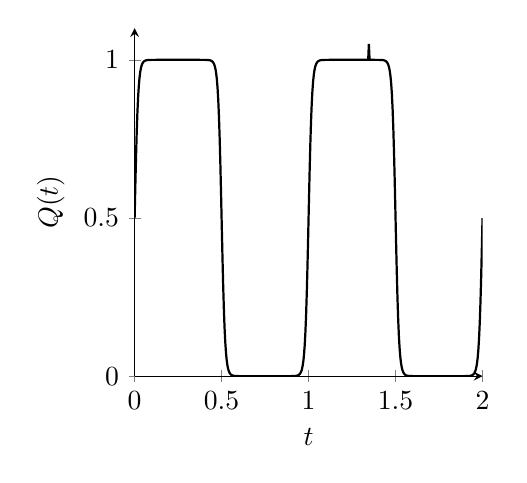
\begin{tikzpicture}
\begin{axis}[
    width=6cm,
    height=6cm,
    xlabel={$t$},
    ylabel={$Q(t)$},
    xmin=0, xmax=2,
    ymin=0, ymax=1.1,
    axis lines=left,
    samples=500,
    domain=0:2,
]

\addplot[
    thick,
]
{
    0.5*(1 + tanh(8*sin(deg(2*pi*x))))
};

\end{axis}
\end{tikzpicture}
\end{center}



Note


\newpage

\subsection*{The Elasticity Module E}
\textcolor{red}{How are we going to implement the elasticity module?}

{\Large Approaches}
\begin{itemize}
	\item Define spring constants $l_{ij}, k_{ij}$ as in the introduction. Derive elasticity module from there.
	\item Define a proper elasticity module carrying the information of the springs. Derive the equation by discretizization of $E$. \{textcolor{blue}{my favorite}.
\end{itemize}

Nonlinear, non-constant. How do we implement E?









\newpage




\chapter{Mathematische Modellierung - Eck, Garcke, Knabner}
\textbf{was möchte ich hiervon wissen?} $\rightarrow$ Wie entstehen Wellen in der Modellierung bei Kontinuumsmechanik? Was für ein Setting bei FilaminC bräuchte man, um das entstehen von Calcium Waves intracellulär mitzunehmen?


%%%%%%%%%%%%					Vom Modell zur Differentialgleichung				%%%%%%%%%%%%%
\subsection*{Vom Modell zur Differentialgleichung}
In diesen drei motivierendenden Beispielen geht es darum, nachzuvollziehen wie aus einer Modellannahme eine Differentialgleichung gefolgert werden kann. Zuerst beschäftigen wir uns mit dem einfachen Fall der Populationsdynamik. Zweitens im Hooksche Gesetze die zu einer ODE führen. Und letzlich um lineare elastizität die uns zu einer PDE führen. So die Hoffnung.





\subsubsection{Populationsmodell}
Im folgenden vollziehen wir Kapitel 1.2 in \cite{EckGarcke2017} nach. \newline 

Ein Bauer hat 200 Rinder. Nach einem Jahr stellt er fest, dass es nun 230 Rinder sind. Nach wieviel Jahren hat der Bauer 600 Rinder? \newline 

Man kann nun verschiedene Modellannahmen treffen. Möglich sind beispielsweise,
\begin{enumerate}
	\item Der Zuwachs der Herde ist rein zufällig.
	\item Der Zuwachs der Herde ist konstant 30.
	\item Der Zuwachs der Herde hängt \textit{irgendwie} ab von der Größe der Herde.
\end{enumerate}
Wir entscheiden uns für letztere. \textit{Insbesondere gehen wir davon aus, das pro Zeiteinheit und Tier ein konstantes Wachstum vorliegt.} An dieser Stelle sei erwähnt, dass wir auch hätten annehmen können, \dots. Gegeben ist also
\begin{equation*}
	x(t_0) = 200, \quad x(t_1) = 230, \quad t_1 = \text{ein Jahr}, \quad r=\frac{x(t_1)}{x(t_0)} = 1,15 \text{ Zuwachs pro Tier pro Zeiteinheit}
\end{equation*}
Gehen wir nun also davon aus, dass der Zuwachs stets von der aktuellen Zahl der Rinder abhängt, so gilt
\begin{equation*}
	x(t) = r^{\frac{t}{t_1-t_0}} x(t_0) = x(t_1)^{\frac{t}{t_1-t_0}} x(t_0)^{( \frac{t}{t_1 - t_0} - 1)}
\end{equation*}
Zu welchem $t$ gilt also
\begin{equation*}
	x(t) = 600
\end{equation*}
Über logarithmieren kommt man auf $t \sim 6,6$. \newline 

Die Wachstumsrate $r$ hängt in unserer Definition vom Zeitintervall ab. Wie lässt sich $r$ als Funktion in der Zeit beschreiben? Vermuten wir einen linearen Zusammenhang, so folgt
\begin{equation*}
	r = 1 + \delta_t p
\end{equation*}
für einen zu bestimmenden Faktor $p>0$. Man sieht leicht, dass hiermit das Herdenwachstum linear beschrieben wäre. Das kann also nicht stimmen.
\textcolor{red}{wieso scheitert dieses lineare wachstum?}

Nehmen wir stattdessen an, dass diese Annahme für sehr kleine $\delta_t$ gilt, erhalten wir 
\begin{equation*}
	x(t + \delta_t) \approx (1+ \delta_t p) x(t)
\end{equation*}
und im Grenzwert
\begin{equation*}
	\lim_{\delta_t \searrow 0} \frac{x(t + \delta_t) - x(t)}{\delta_t}= \partial_t x(t) = p x(t)
\end{equation*}
Diese \textit{gewöhnlich Differentialgleichung} besitzt die exakte Lösung
\begin{equation*}
	x(t) = x(t_0) e^{(p(t - t_0))}
\end{equation*}
Über die Bedingung
\begin{equation*}
	e^{p \cdot \text{ ein Jahr}} = 1,15
\end{equation*}
erhält man den exakten Wert für $p$.

Weiterhin wird gezeigt, dass das diskrete Model $x(t_{n+1}) = r x(t_n)$ in einer art und weise "genau" ist (impliziter und expliziter euler).

\subsection{Stabwerke}





\subsection*{Space frames or Stabwerke}
\begin{definition}[Elastisch]\cite[p.49]{EckGarcke2017} An object is called \textit{elastic} if, once force is not applied anymore, it goes back in its original state.
\end{definition}
Hier gibt es drei Beispiele zu Stabwerken die modelliert werden. Unter den Modellannahmen, insbesondere der geometrischen Linearisierung, führen diese Modell zu linearen Gleichungssystemen, die die Auslenkung beschreiben.

\subsection*{Ordinary Differential equations}
Hängen die relevanten Größen nur von einer Variable ab, erhält man eine gewöhnliche Differentialgleichung.

\subsubsection*{Eindimensionale Schwingungen}
Ein an einer Feder befestigter Massepunkt der Masse $m$. 
\begin{equation*}
	m \ddot{x} = F
\end{equation*}
Im einfachsten Fall ist die Kraft linear zur Auslenkung. Beschrieben über die Federkonstante $k$,
\begin{equation*}
	F_F = -k x
\end{equation*}
Auf Seite p.141 wird diese etwas erweitert mit rückstellkraft und visköser Dämpfung zu
\begin{equation*}
	m \ddot{x} + \beta \dot{x} + kx = f
\end{equation*}
mit beliebiger zeitabhängiger rechter Seite $f$.

